% One-page poster. Build: tectonic poster/poster.tex
\documentclass[12pt]{article}
\usepackage[paperwidth=46.2cm,paperheight=37.8cm,margin=1.5cm,top=1.2cm]{geometry}
\usepackage{lmodern}
\usepackage[T1]{fontenc}
\usepackage{amsmath}
\usepackage{booktabs}
\usepackage{xcolor}
\usepackage{enumitem}
\usepackage{caption}
\usepackage{tikz}
\usepackage{pgfplots}
\pgfplotsset{compat=1.18}
\usetikzlibrary{positioning,arrows.meta,calc,fit}

\definecolor{accent}{RGB}{28,50,120}
\definecolor{soft}{RGB}{236,239,246}
\pagestyle{empty}
\newlength{\colh}\setlength{\colh}{31cm}
\setlength{\parindent}{0pt}
\setlength{\parskip}{6pt}
\captionsetup{font=small,labelfont=bf,skip=6pt}
\setlist[itemize]{leftmargin=1.2em,itemsep=3pt,topsep=2pt}

\newcommand{\firsthead}[1]{{\Large\bfseries\color{accent}#1}\par\vspace{2pt}}
\newcommand{\head}[1]{\vspace{10pt plus 1fil}\firsthead{#1}}
\tikzset{
  box/.style={draw,rectangle,minimum height=0.9cm,inner sep=5pt,align=center,font=\small},
  key/.style={box,fill=soft},
  arr/.style={-{Latex[length=2.2mm]},thick},
}

\begin{document}

\begin{center}
{\fontsize{40}{48}\selectfont\bfseries\color{accent} Two-Stage Product Search Ranker}\par\vspace{8pt}
{\Large Hybrid retrieval and a cascade of rankers for the Shopping Queries (ESCI) dataset}
\end{center}
\vspace{14pt}

\begin{minipage}[t][\colh][s]{0.31\textwidth}
\firsthead{Task}
Given a shopping query, rank products from a 482k catalog so that exact matches come first.
The whole search must answer within 100\,ms.
Every labelled query-product pair carries one of four ESCI labels, and each label has a gain.

\begin{center}
\begin{tabular}{llcc}
\toprule
 & Label & Gain & Share \\
\midrule
E & Exact: matches the query & 1.0 & 43.5\% \\
S & Substitute: some detail differs & 0.1 & 35.1\% \\
C & Complement: goes with it & 0.01 & 4.5\% \\
I & Irrelevant & 0 & 16.9\% \\
\bottomrule
\end{tabular}
\captionof{table}{ESCI labels on the US English data.}
\end{center}

\head{Data}
We use the US English part of task 1: 29.8k queries and 601k labelled pairs.
Queries are split, never rows, so no query sits in two splits.
The cross-encoder trains on its own queries, so LightGBM never learns from scores the cross-encoder made on its own training data.

\begin{center}
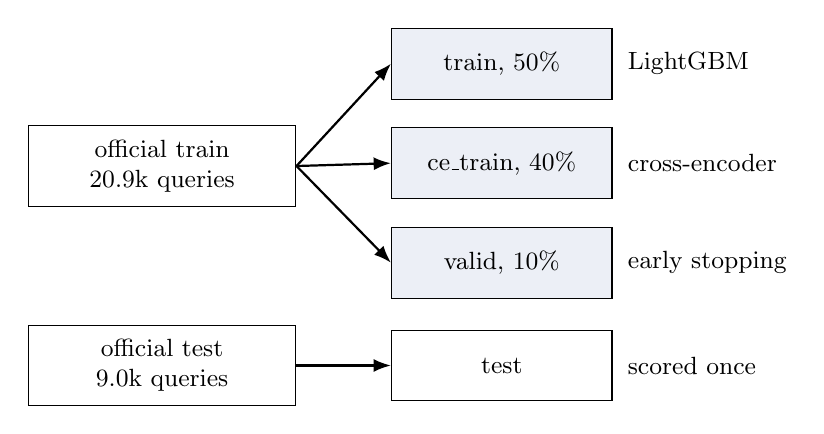
\begin{tikzpicture}[node distance=0.35cm and 1.2cm]
  \node[box,minimum width=3.4cm] (tr) {official train\\20.9k queries};
  \node[key,minimum width=2.8cm,right=of tr,yshift=1.3cm] (a) {train, 50\%};
  \node[key,minimum width=2.8cm,below=of a] (b) {ce\_train, 40\%};
  \node[key,minimum width=2.8cm,below=of b] (c) {valid, 10\%};
  \node[box,minimum width=3.4cm,below=1.5cm of tr] (te) {official test\\9.0k queries};
  \node[box,minimum width=2.8cm] (t) at (te -| c) {test};
  \foreach \n in {a,b,c} \draw[arr] (tr.east) -- (\n.west);
  \draw[arr] (te) -- (t);
  \node[right=2pt of a,font=\small] {LightGBM};
  \node[right=2pt of b,font=\small] {cross-encoder};
  \node[right=2pt of c,font=\small] {early stopping};
  \node[right=2pt of t,font=\small] {scored once};
\end{tikzpicture}
\captionof{figure}{Query-level split.}
\end{center}

\head{Metrics}
With $g_i$ the gain of the product at rank $i$,
\[
\mathrm{DCG@}k=\sum_{i=1}^{k}\frac{g_i}{\log_2(i+1)},\qquad
\mathrm{NDCG@}k=\frac{\mathrm{DCG@}k}{\mathrm{IDCG@}k}.
\]
\textbf{Full-list NDCG} takes $k$ as each query's whole labelled list, as the KDD Cup leaderboard did.
\textbf{NDCG@10} looks only at what a shopper sees, and is much stricter.
\textbf{Recall@}$k$ is the share of Exact products that retrieval finds in its top $k$ of the whole catalog.

\head{Latency}
500 test queries replayed one at a time through the HTTP API, on an Apple M4 Pro laptop.

\begin{center}
\begin{tabular}{lrr}
\toprule
Stage & p50 (ms) & p95 (ms) \\
\midrule
Encode query & 4.7 & 5.3 \\
Retrieve 200 candidates & 3.0 & 4.8 \\
Features for 200 & 14.7 & 18.2 \\
Light ranker & 0.6 & 0.7 \\
Cross-encoder on top 50 & 19.2 & 22.2 \\
Full ranker & 0.6 & 0.8 \\
\midrule
Total, including HTTP & \textbf{44.7} & \textbf{49.9} \\
\bottomrule
\end{tabular}
\captionof{table}{Per-stage latency.}
\end{center}
\end{minipage}\hfill
\begin{minipage}[t][\colh][s]{0.31\textwidth}
\firsthead{System}
Stage one recalls candidates cheaply from the whole catalog.
Stage two spends more compute on fewer products: a light ranker sorts all 200 candidates, and only its top 50 reach the cross-encoder.

\begin{center}
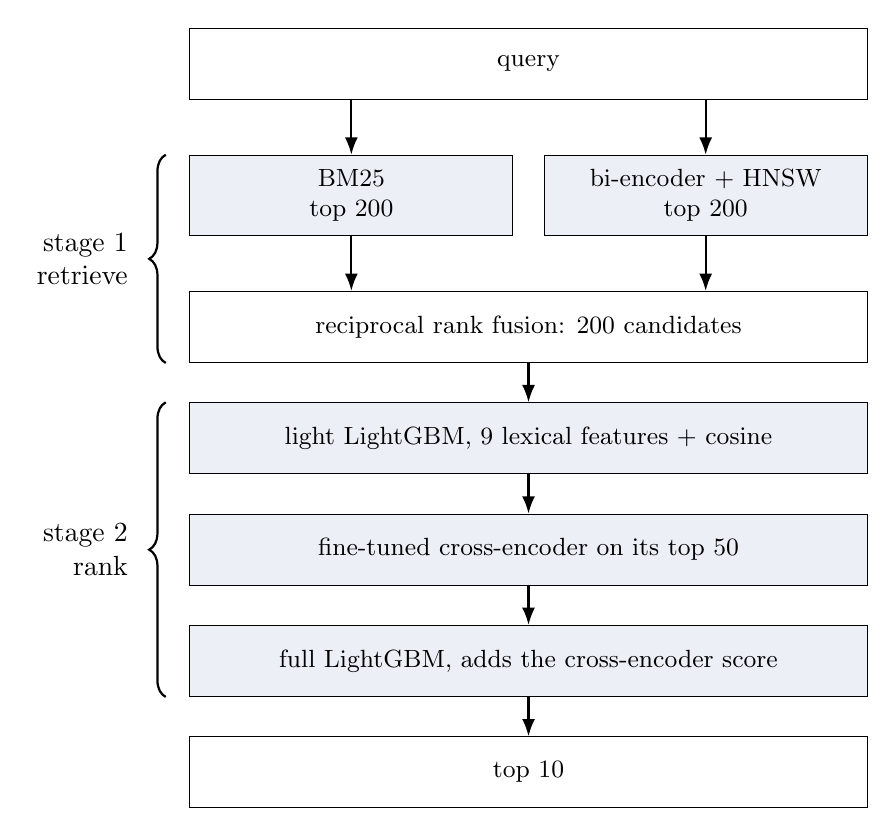
\begin{tikzpicture}[node distance=0.5cm, every node/.append style={font=\normalsize}]
  \def\W{8.6cm}
  \node[box,minimum width=\W] (q) {query};
  \node[key,minimum width=4.1cm,below=0.7cm of q.south west,anchor=north west] (bm) {BM25\\top 200};
  \node[key,minimum width=4.1cm,below=0.7cm of q.south east,anchor=north east] (de) {bi-encoder + HNSW\\top 200};
  \node[box,minimum width=\W,below=0.7cm of bm.south west,anchor=north west] (rrf) {reciprocal rank fusion: 200 candidates};
  \node[key,minimum width=\W,below=of rrf] (li) {light LightGBM, 9 lexical features + cosine};
  \node[key,minimum width=\W,below=of li] (ce) {fine-tuned cross-encoder on its top 50};
  \node[key,minimum width=\W,below=of ce] (fu) {full LightGBM, adds the cross-encoder score};
  \node[box,minimum width=\W,below=of fu] (out) {top 10};
  \draw[arr] (bm.north |- q.south) -- (bm); \draw[arr] (de.north |- q.south) -- (de);
  \draw[arr] (bm) -- (bm |- rrf.north); \draw[arr] (de) -- (de |- rrf.north);
  \foreach \a/\b in {rrf/li,li/ce,ce/fu,fu/out} \draw[arr] (\a) -- (\b);
  \draw[decorate,decoration={brace,amplitude=6pt},thick] ($(rrf.south west)+(-0.3,0)$) -- ($(bm.north west)+(-0.3,0)$)
    node[midway,left=10pt,align=right] {stage 1\\retrieve};
  \draw[decorate,decoration={brace,amplitude=6pt},thick] ($(fu.south west)+(-0.3,0)$) -- ($(li.north west)+(-0.3,0)$)
    node[midway,left=10pt,align=right] {stage 2\\rank};
\end{tikzpicture}
\captionof{figure}{Online serving cascade.}
\end{center}

\head{Cross-encoder}
A bi-encoder embeds query and product separately.
A cross-encoder reads them together, so every query token attends to every title token.
We fine-tune \texttt{ms-marco-MiniLM-L6} (22M parameters) for one epoch on 8.3k ce\_train queries, about 5 minutes on the laptop GPU.
The target is the ESCI gain itself, so Substitutes count as partly relevant.

\begin{center}
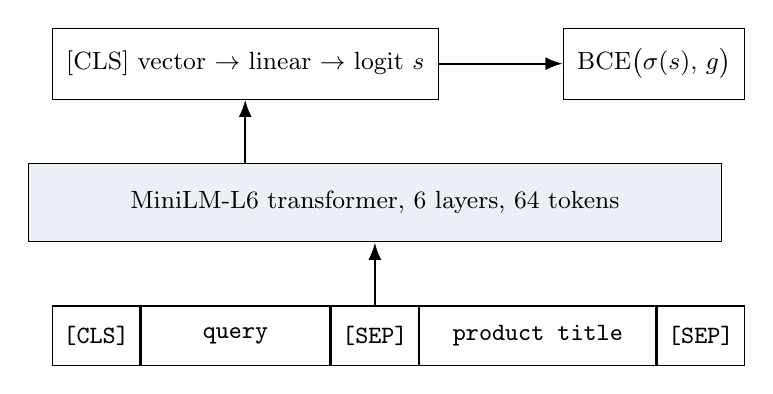
\begin{tikzpicture}[tok/.style={draw,minimum height=0.75cm,inner sep=4pt,font=\small\ttfamily}]
  \node[tok] (t1) {[CLS]};
  \node[tok,right=0pt of t1,minimum width=2.4cm] (t2) {query};
  \node[tok,right=0pt of t2] (t3) {[SEP]};
  \node[tok,right=0pt of t3,minimum width=3.0cm] (t4) {product title};
  \node[tok,right=0pt of t4] (t5) {[SEP]};
  \path let \p1=(t1.west), \p2=(t5.east) in
    node[key,minimum width=\x2-\x1,minimum height=1.0cm,above=0.8cm of t3.north,anchor=south] (enc) {MiniLM-L6 transformer, 6 layers, 64 tokens};
  \node[box,above=0.8cm of enc.north -| t1.west,anchor=south west] (cls) {[CLS] vector $\rightarrow$ linear $\rightarrow$ logit $s$};
  \node[box,above=0.8cm of enc.north -| t5.east,anchor=south east] (loss) {BCE$\big(\sigma(s),\,g\big)$};
  \draw[arr] (t3.north) -- (enc.south);
  \draw[arr] (enc.north -| cls) -- (cls.south);
  \draw[arr] (cls) -- (loss);
\end{tikzpicture}
\captionof{figure}{Cross-encoder input and training target $g\in\{1,0.1,0.01,0\}$.}
\end{center}

\begin{center}
\begin{tabular}{lcc}
\toprule
Cross-encoder & NDCG@10 & Full NDCG \\
\midrule
Zero-shot, alone & 0.719 & 0.836 \\
Fine-tuned, alone & 0.750 & 0.853 \\
Fine-tuned, inside full LightGBM & \textbf{0.759} & \textbf{0.858} \\
\bottomrule
\end{tabular}
\captionof{table}{Effect of fine-tuning, test split.}
\end{center}
\end{minipage}\hfill
\begin{minipage}[t][\colh][s]{0.31\textwidth}
\firsthead{Results}
Each idea, added in turn and scored on the untouched official test split.
On the competition's full-list metric the system reaches 0.858, above the official 0.83 baseline.

\begin{center}
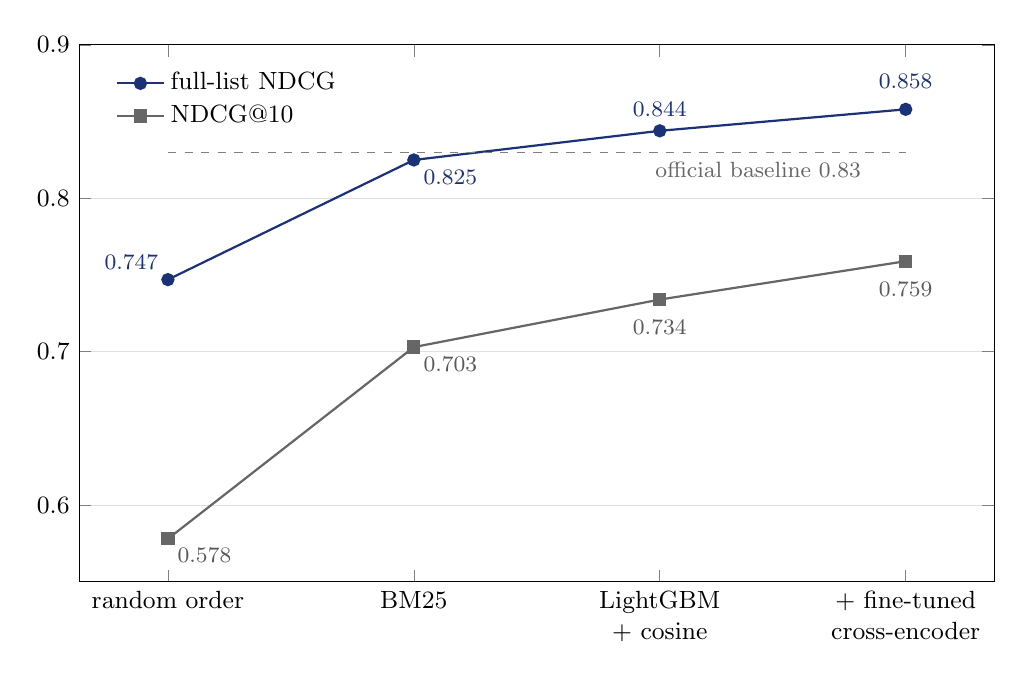
\begin{tikzpicture}
\begin{axis}[
  width=13.2cm, height=8.4cm,
  symbolic x coords={Random,BM25,LightGBM,+ CE},
  xtick=data, xticklabels={random order, BM25, {LightGBM\\+ cosine}, {+ fine-tuned\\cross-encoder}},
  xticklabel style={align=center,font=\small},
  ymin=0.55, ymax=0.9, ytick={0.6,0.7,0.8,0.9},
  yticklabel style={font=\small,/pgf/number format/fixed,/pgf/number format/precision=1},
  ymajorgrids, grid style={gray!25},
  enlarge x limits=0.12,
  legend style={at={(0.03,0.97)},anchor=north west,font=\small,draw=none,fill=white},
  legend cell align=left,
]
\addplot[accent,thick,mark=*] coordinates {(Random,0.747) (BM25,0.825) (LightGBM,0.844) (+ CE,0.858)};
\addplot[black!60,thick,mark=square*] coordinates {(Random,0.578) (BM25,0.703) (LightGBM,0.734) (+ CE,0.759)};
\draw[dashed,black!50] (axis cs:Random,0.83) -- (axis cs:+ CE,0.83) node[pos=0.8,below,font=\footnotesize,text=black!60] {official baseline 0.83};
\begin{scope}[font=\footnotesize]
  \node[text=accent,anchor=south east] at (axis cs:Random,0.747) {0.747};
  \node[text=accent,anchor=north west] at (axis cs:BM25,0.825) {0.825};
  \node[text=accent,anchor=south,yshift=4pt,fill=white,inner sep=1pt] at (axis cs:LightGBM,0.844) {0.844};
  \node[text=accent,anchor=south,yshift=4pt] at (axis cs:+ CE,0.858) {0.858};
  \node[text=black!65,anchor=north west] at (axis cs:Random,0.578) {0.578};
  \node[text=black!65,anchor=north west] at (axis cs:BM25,0.703) {0.703};
  \node[text=black!65,anchor=north,yshift=-4pt] at (axis cs:LightGBM,0.734) {0.734};
  \node[text=black!65,anchor=north,yshift=-4pt] at (axis cs:+ CE,0.759) {0.759};
\end{scope}
\legend{full-list NDCG, NDCG@10}
\end{axis}
\end{tikzpicture}
\captionof{figure}{NDCG on the official test split. The dashed line is the official baseline on the full-list metric.}
\end{center}

Lexical features stop helping around 0.725 NDCG@10.
What is left is mostly telling Exact from Substitute when the words overlap, which needs a model that reads both texts.

\begin{center}
\begin{tabular}{lcc}
\toprule
Retrieval, 482k products & R@100 & R@200 \\
\midrule
BM25 & 0.578 & 0.652 \\
Bi-encoder + HNSW & 0.518 & 0.598 \\
Hybrid, RRF & \textbf{0.628} & \textbf{0.697} \\
\bottomrule
\end{tabular}
\captionof{table}{Recall of Exact products.}
\end{center}

Searching the whole catalog end to end, the top 10 scores 0.372 NDCG@10, against 0.317 for BM25 alone.
Unlabelled products count as 0, so this is a lower bound.

\head{Monitoring}
Requests are logged and compared with a reference by population stability index (PSI).
Above 0.25 counts as drift.

\begin{center}
\begin{tabular}{lcc}
\toprule
Traffic & Query length & Top score \\
\midrule
Replayed test queries & 0.001 & 0.059 \\
Spanish queries & 0.093 & \textbf{1.086} \\
\bottomrule
\end{tabular}
\captionof{table}{PSI on an input and an output signal.}
\end{center}

\head{Summary}
\begin{itemize}
  \item BM25 and dense retrieval miss different products, so fusing them finds 5 points more Exact products.
  \item The fine-tuned cross-encoder gives the largest single gain, and takes 68\% of the full ranker's split gain.
  \item Running it only on the light ranker's top 50 keeps p95 latency at 50\,ms.
  \item An input-only monitor would have missed the Spanish traffic. The output score caught it.
\end{itemize}
\end{minipage}

\end{document}
